%!TEX root = ULL_thesis_template.tex 
\chapter{Using Input Shaping to Validate RL Controllers}
\label{chapter3}
%
In utilizing RL to define a control strategy for a robotic system, the resulting commands sent to the system are often described as optimal, or at least approaching optimal. They are described as such due to the nature of RL problems in that the techniques used to learn a policy are optimization-theory based, so the policy being trained is one that is approaching an optimal solution in regards to the reward defined. Interpreting the commands claimed to be optimal, in the context of control theory, is an important part of utilizing RL for defining control strategies for robotic systems. In the case of a flexible jumping robot, where the command is to jump the system as high as possible or as efficiently as possible, the questions arises if the commands generated truly approach an optimal solution or not. To answer this question, the commands resulting from the trained agents can be analyzed leveraging conventional control theory. Methods such as input shaping have been shown to be effective for defining optimal control strategies for flexible jumping systems and can be used to evaluate the commands generated by the RL generated policies \cite{Vaughan2013}.

%%%%%%%%%%%%%%%%%%%%%%%%%%%%%%%%%%%%%%%%%%%%%%%%%%%%%%%%%%%%%%%%%%%%%%%%
%%%%%%%%%%%%%%%%%%%%%%%%%%%%%%%%%%%%%%%%%%%%%%%%%%%%%%%%%%%%%%%%%%%%%%%%
\section{Input Shaping Controller Input}
\label{sec:controller_input}
Bang-bang-based jumping commands like the one shown in Figure~\ref{fig:commandForm} are likely to result in a maximized jump height \cite{Vaughan2013}. For these command types, regarding the monopode jumping system, the actuator mass travels at maximum acceleration within its allowable range, pauses, then accelerates in the opposite direction. Commands designed to complete this motion are bang-bang in each direction, with a selectable delay between them. The resulting motion of the actuator along the rod is shown in Figure~\ref{fig:jumpingCommandPosition}. Starting from an initial position, $x_{a_0}$, the actuator moves through a motion of stroke length $\Delta_1$, pauses there for $\delta_t$, then moves a distance $\Delta_2$ during the second portion of the acceleration input.
%
\begin{figure}[tb!]
\centering
    \begin{subfigure}{0.45\columnwidth}
    \centering
    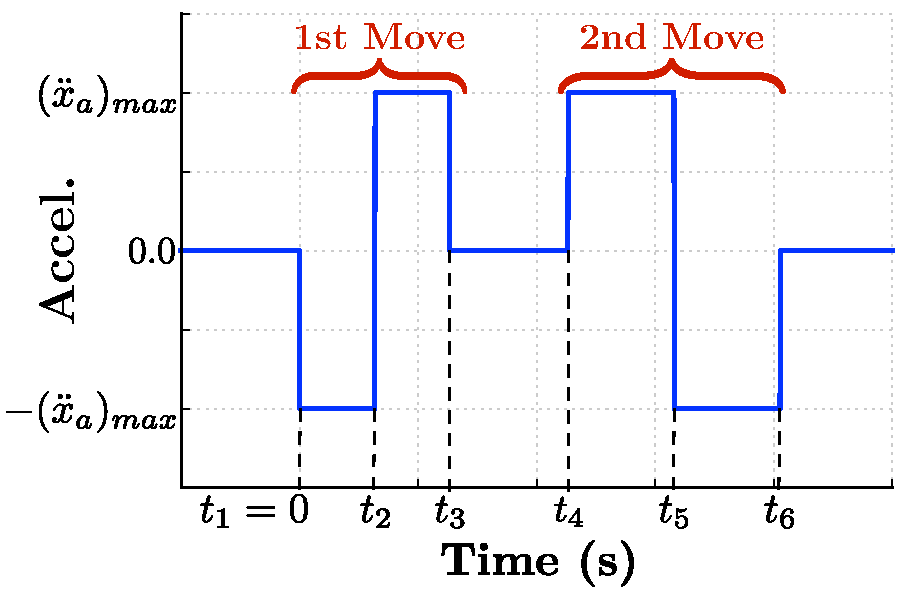
\includegraphics[width=\columnwidth]{Figures/Ch3/input_shaping/Command_form.pdf}
    \caption{Jumping Command \cite{Vaughan2013}}
    \label{fig:commandForm}
    \end{subfigure}
%
\hspace{0.05\columnwidth} % Optionally add some space between side-by-side figs
%
    \begin{subfigure}{0.45\columnwidth}
    \centering
    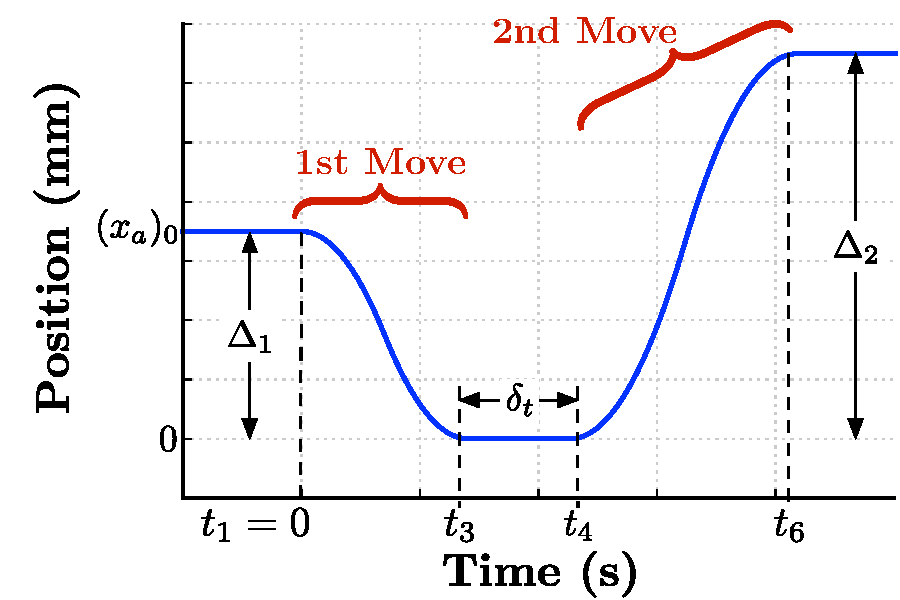
\includegraphics[width=\columnwidth]{Figures/Ch3/input_shaping/Jumping_command_position.pdf}
    \caption{Resulting Actuator Motion \cite{Vaughan2013}}
    \label{fig:jumpingCommandPosition}
    \end{subfigure}
\caption{Jumping Command Profiles} % Full figure caption
\label{fig:jumping_commands}	% Full figure label
\end{figure}
%

This bang-bang-based profile can be represented as a step command convolved with a series of impulses, as is shown in Figure \ref{fig:jumpConvolve} \cite{Sorensen2008CommandinducedVA}. Using this decomposition, input-shaping principles and tools can be used to both analyze and design the impulse sequence \cite{Singer:90, Singhose:94a}. For the bang-bang-based jumping command shown in Figure~\ref{fig:jumpConvolve}, the amplitudes of the resulting impulse sequence are fixed, $A_i = [-1, 2, -1, 1, -2, 1]$. The impulse times, $t_i$, can be varied and optimized leading to a maximized jump height of the monopode system \cite{Vaughan2013}. Commands of this form will often result in a stutter jump, like what was shown in Figure~\ref{fig:stutterJump} of Chapter~\ref{chapter2}, where the small initial jump allows the system to compress the spring to store energy to be used in the final jump. 
%
\begin{figure}[tb!]
  \centering
    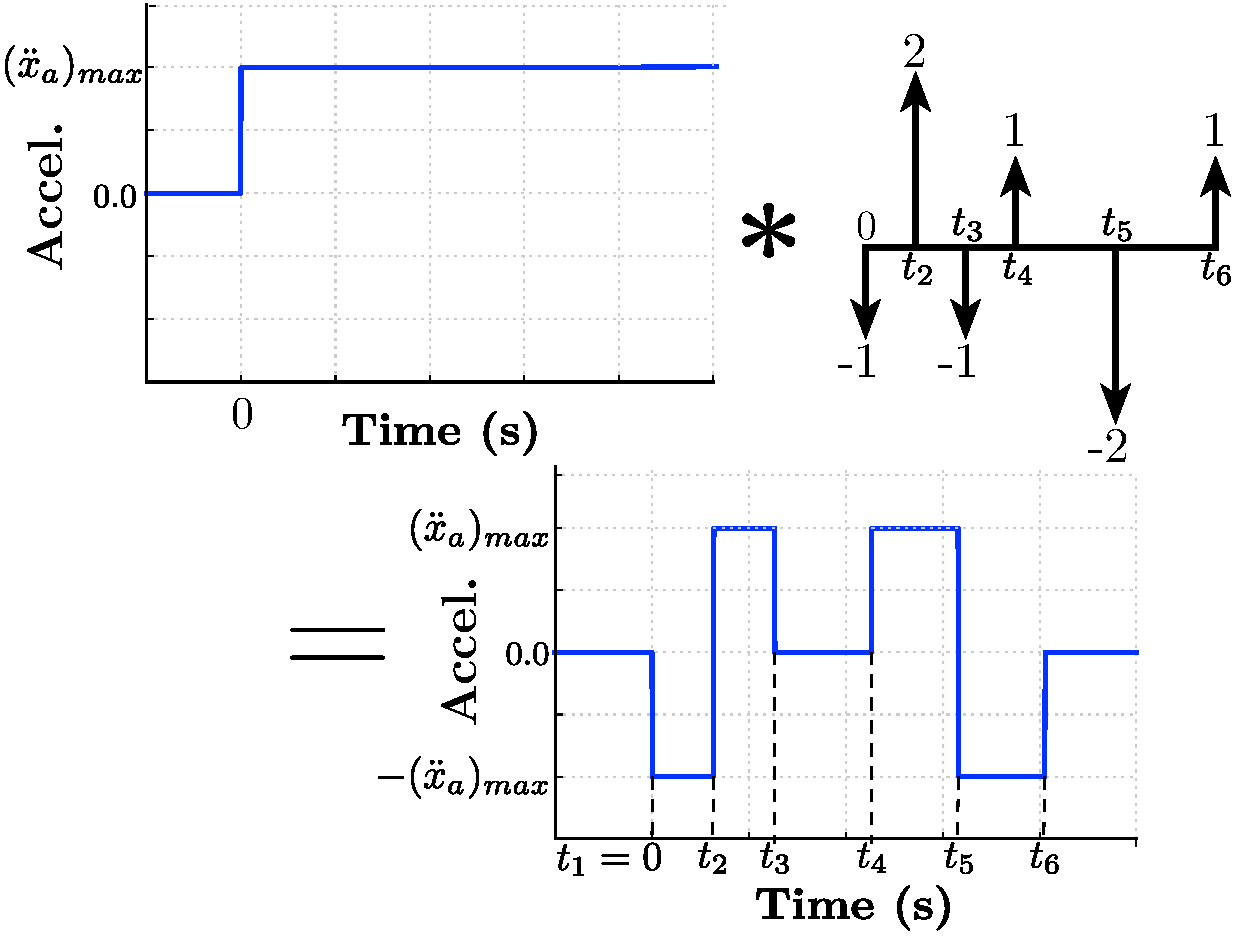
\includegraphics[width=0.75\textwidth]{Figures/Ch3/input_shaping/Jump_convolve.pdf}
    \caption{Decomposition of the Jump Command into a Step Convolved with an Impulse Sequence \cite{Vaughan2013}}
    \label{fig:jumpConvolve}
\end{figure}
%


%%%%%%%%%%%%%%%%%%%%%%%%%%%%%%%%%%%%%%%%%%%%%%%%%%%%%%%%%%%%%%%%%%%%%%%%
%%%%%%%%%%%%%%%%%%%%%%%%%%%%%%%%%%%%%%%%%%%%%%%%%%%%%%%%%%%%%%%%%%%%%%%%
\section{Review of Vector Diagrams}
\label{sec:vector_diagram_review}
%
One tool that seeks to simplify the design of impulse sequences for input shapers is the vector diagram \cite{Singhose:94a}. The vector diagram represents the vibration caused by an impulse as a vector, and the vibration induced by an impulse sequence as the sum of the representative vectors of the sequence. As such, the vector diagram can provide a visual means of both analysis and design of impulse sequences.

The process of plotting an impulse sequence on a vector diagram is shown in Figure~\ref{fig:vector_2imp}. 
%
\begin{figure}[tb!]
\begin{center}
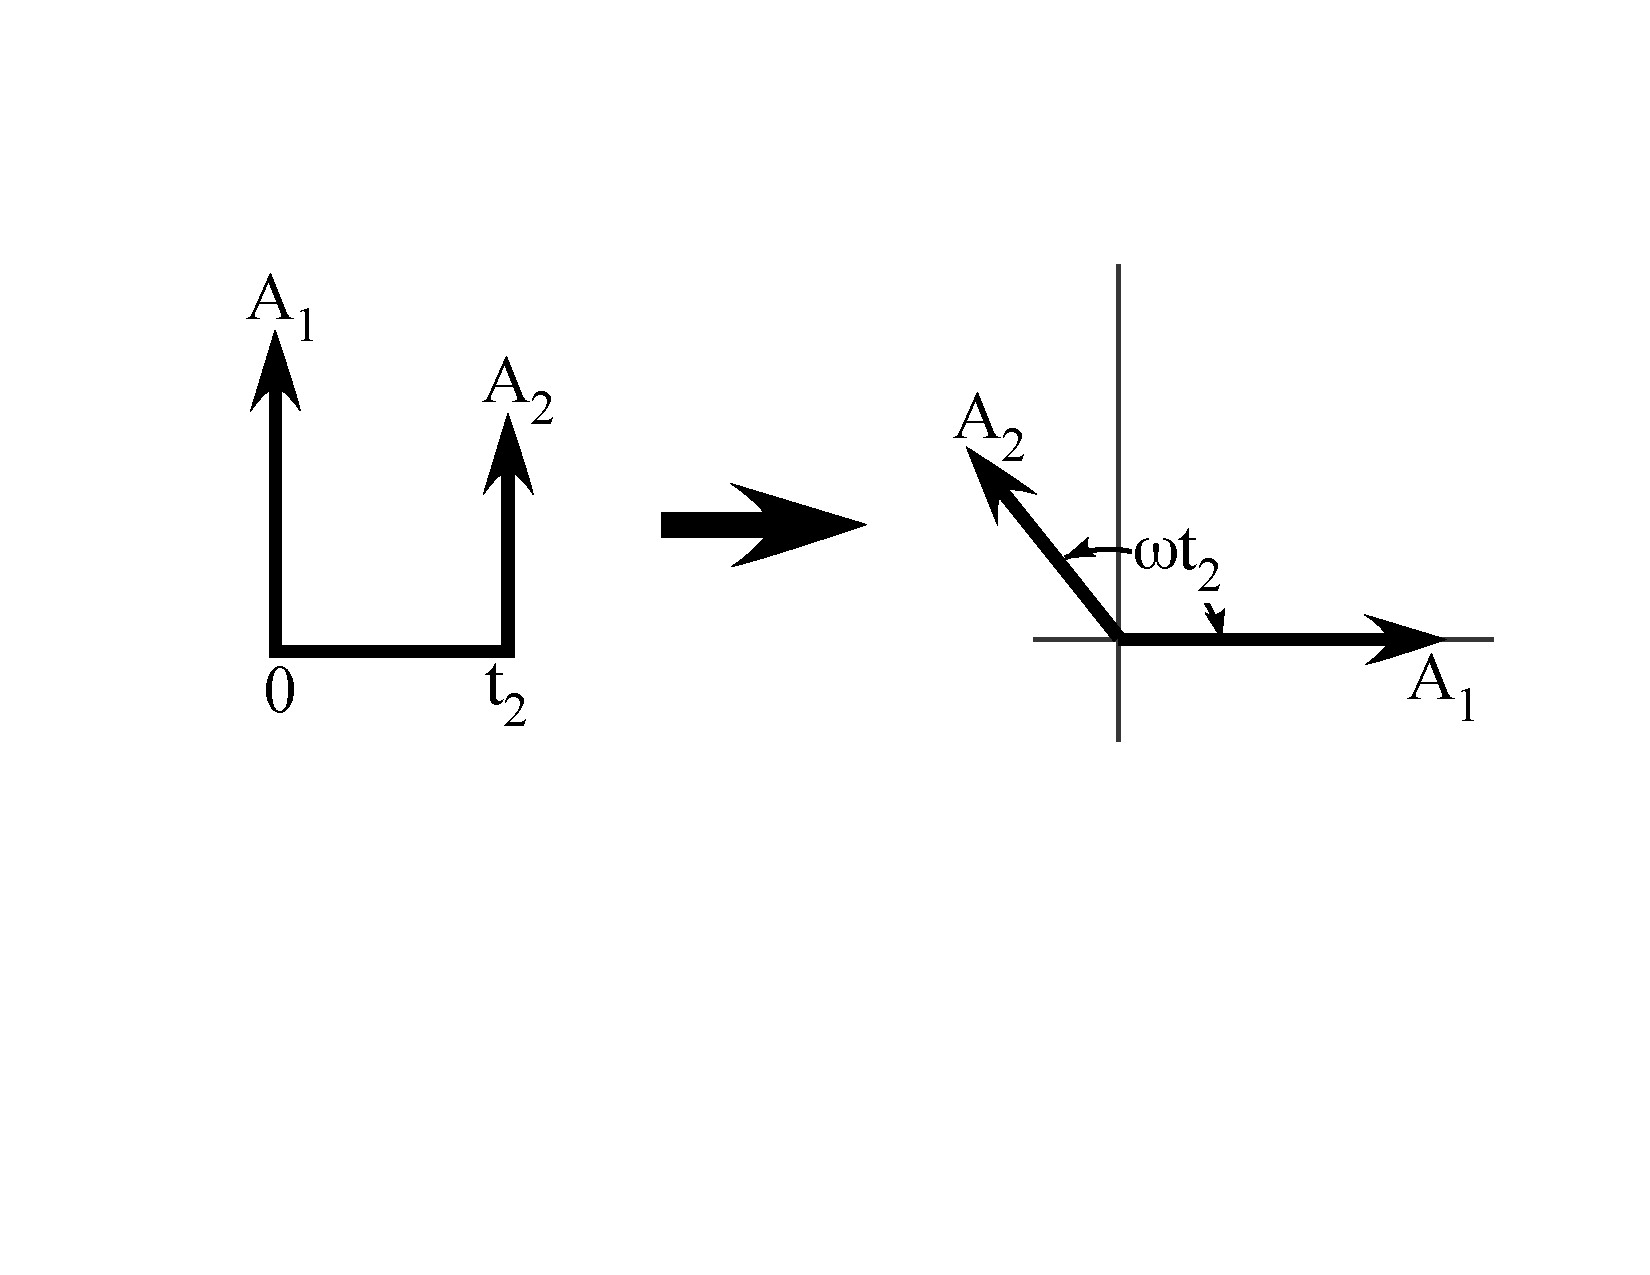
\includegraphics[width = 4.5in]{Figures/Ch3/input_shaping/vector_diagram_2imp}
\caption{Plotting Impulses on a Vector Diagram}
\label{fig:vector_2imp}
\end{center}
\end{figure}
%
Each impulse is plotted on the vector diagram in polar coordinates, where the magnitude of each vector is simply the impulse magnitude, and its angle is $\theta = \omega t_i$, where $\omega$ is the system natural frequency, and $t_i$ is the time location of the impulse.

To calculate the residual vibration caused by a sequence of impulses, the representative vectors are summed, as shown in Figure \ref{fig:vector_result}. 
%
\begin{figure}[tb!]
\begin{center}
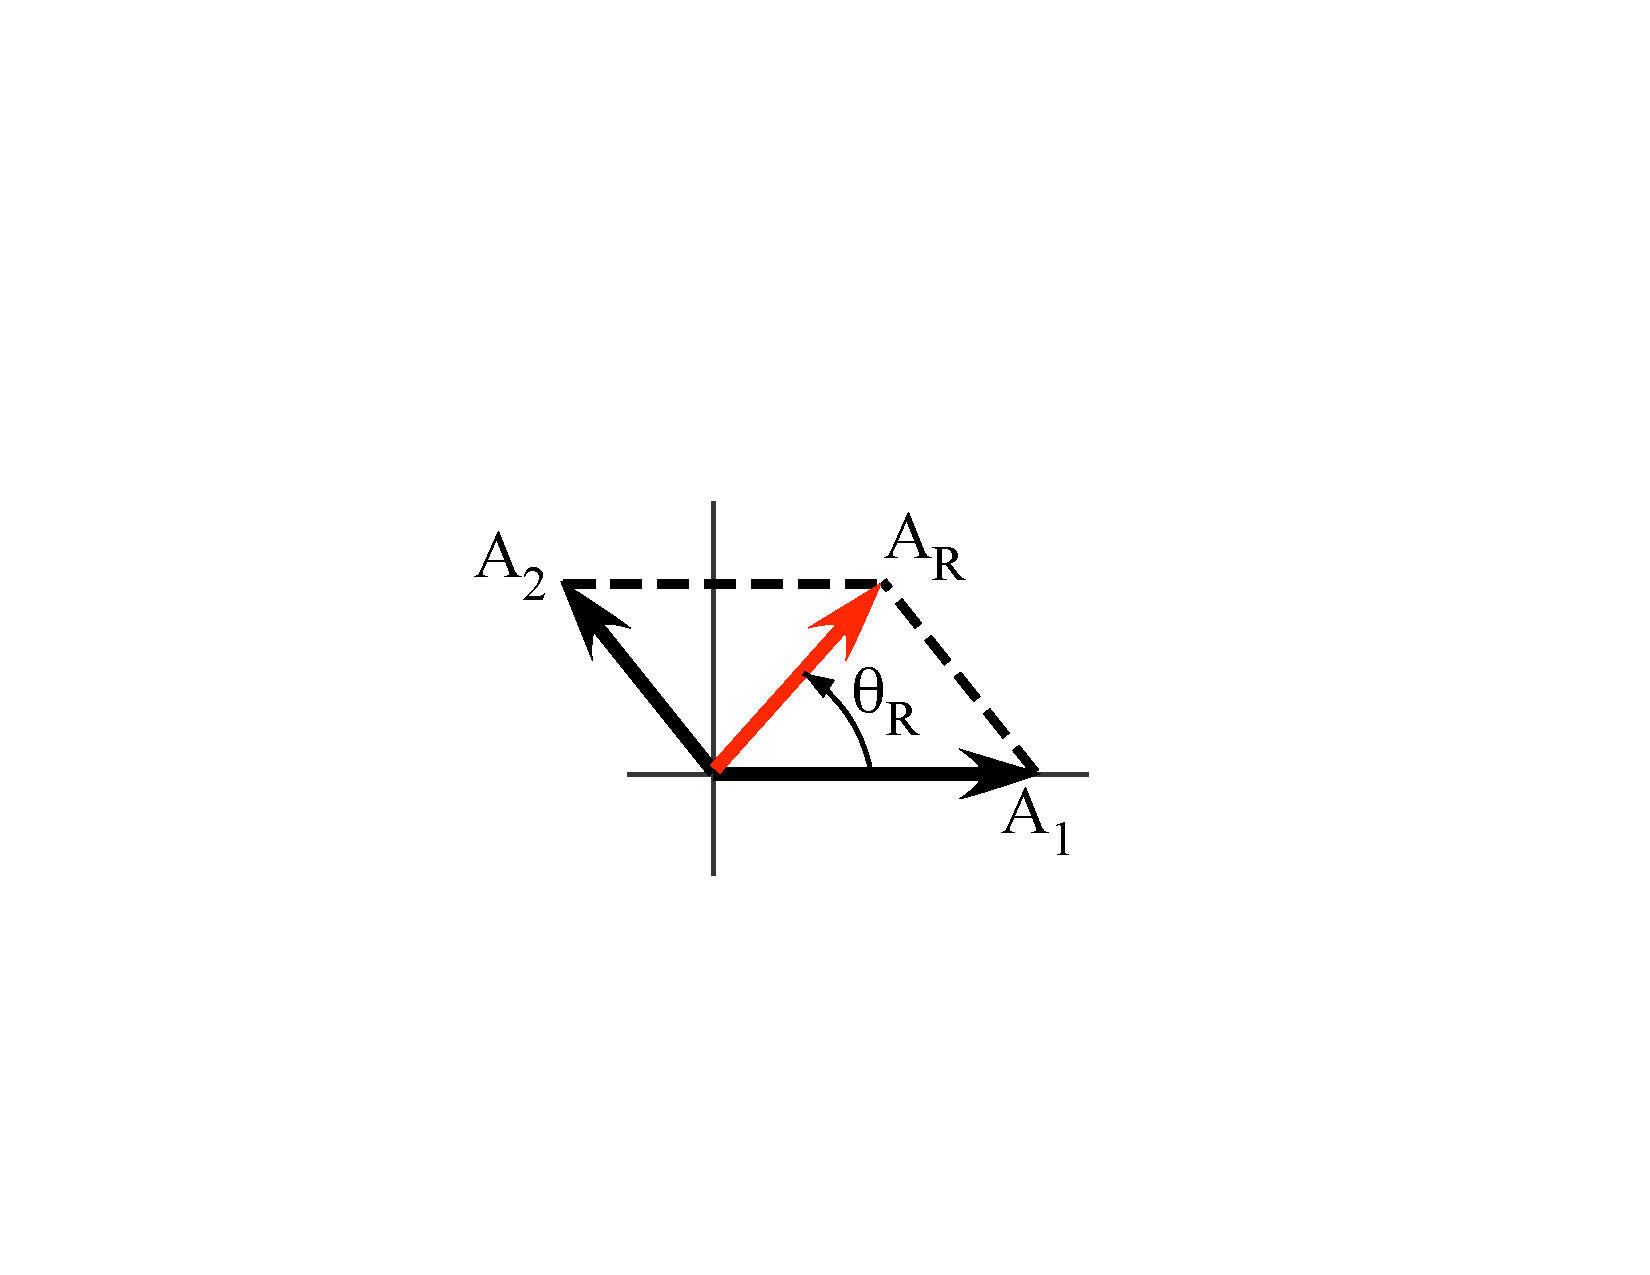
\includegraphics[width = 3in]{Figures/Ch3/input_shaping/vector_diagram_result}
\caption{Resultant Vibration Vector from Adding Impulses}
\label{fig:vector_result}
\end{center}
\end{figure}
%
The magnitude of the residual vibration caused by the sequence is proportional to the magnitude of the resultant vector, $A_R$.

The vector diagram can also be used as an input shaper design tool. For example, a third vector can be added to the sequence plotted in Figure \ref{fig:vector_result} to produce zero vibration. This third vector, $A_3$, could be placed opposite of $A_R$, as shown in Figure \ref{fig:vector_design_pos}. When $A_3$ is placed this way, the three vectors in the diagram sum to zero, indicating the impulse sequence will excite zero vibration at the design frequency and damping ratio.

To plot a negative impulse, the vector simply points toward the origin instead of away. Another option to design a zero vibration shaper from Figure \ref{fig:vector_result} is to place a negative impulse at $A_R$, as is shown in Figure \ref{fig:vector_design_neg}.
% 
\begin{figure}[tb!]
  \centering
  \begin{subfigure}[b]{0.45\textwidth}
    \centering
    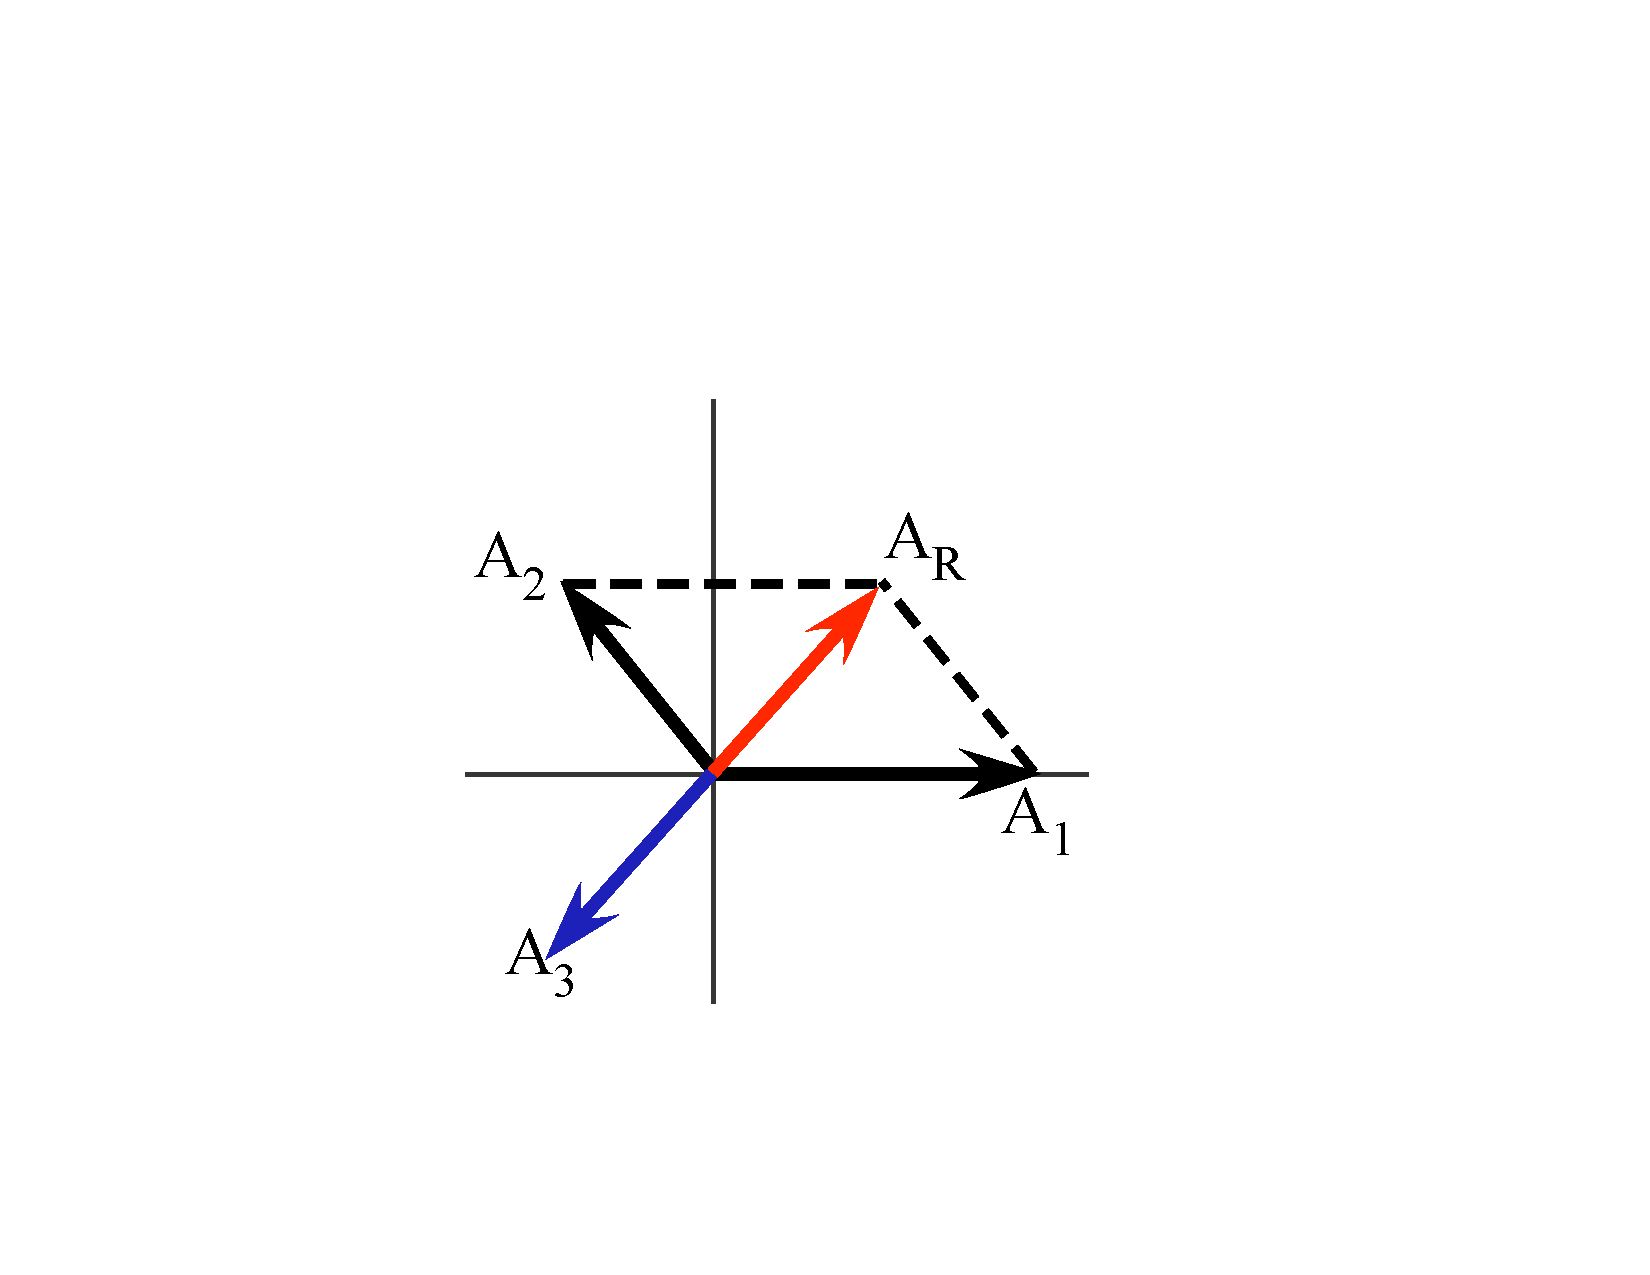
\includegraphics[width=\textwidth]{Figures/Ch3/input_shaping/vector_diagram_design}
    \caption{Adding a Positive Impulse}
    \label{fig:vector_design_pos}
  \end{subfigure}
  \hfill
  \begin{subfigure}[b]{0.45\textwidth}
    \centering
    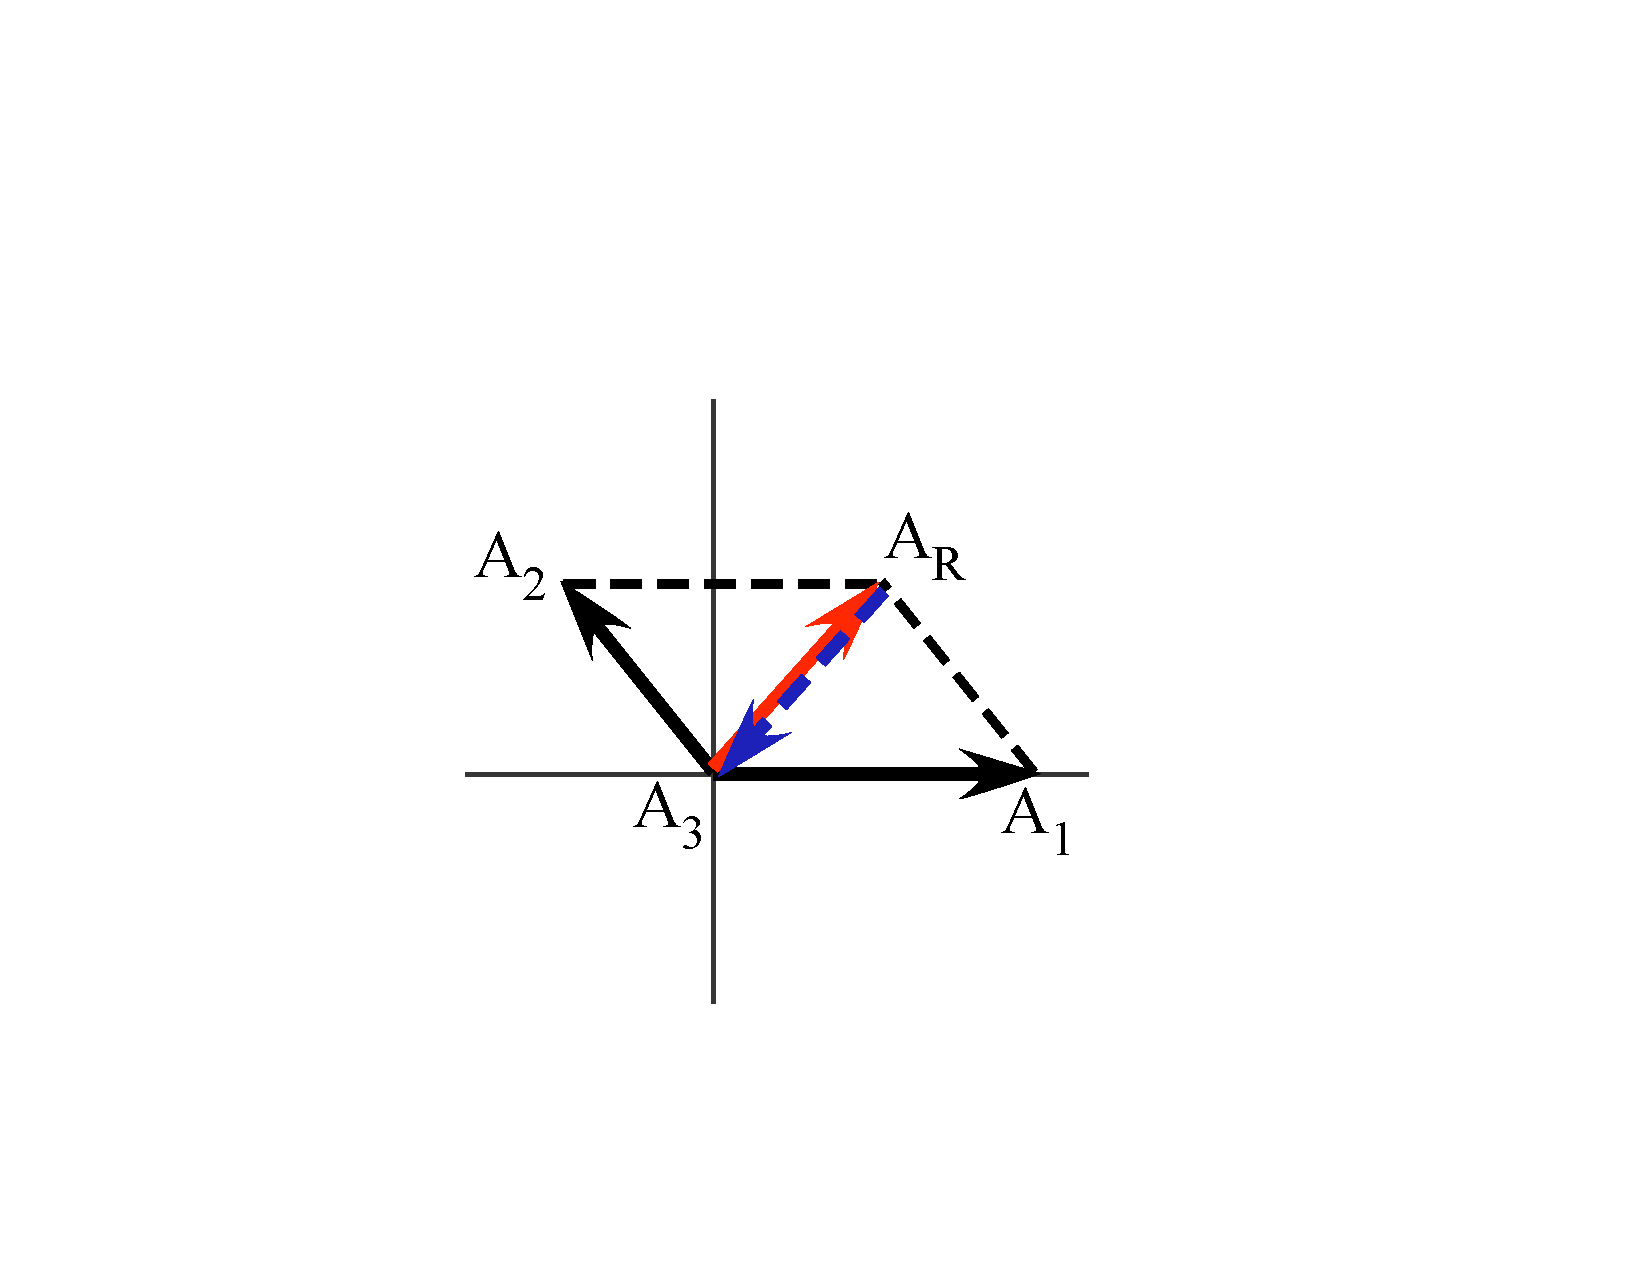
\includegraphics[width=\textwidth]{Figures/Ch3/input_shaping/vector_diagram_design_neg}
     \caption{Adding a Negative Impulse}
     \label{fig:vector_design_neg}
  \end{subfigure}
   \caption{Designing Input Shapers Using Vector Diagrams}
   \label{fig:vector_design}
\end{figure} 

In the context of this work, the vector diagram can be used to design an impulse sequence that \textit{maximizes} vibration. In other words, instead of arranging vectors to force $A_R$ toward zero, the vectors can be arranged to increase its magnitude. 


%%%%%%%%%%%%%%%%%%%%%%%%%%%%%%%%%%%%%%%%%%%%%%%%%%%%%%%%%%%%%%%%%%%%%%%%
%%%%%%%%%%%%%%%%%%%%%%%%%%%%%%%%%%%%%%%%%%%%%%%%%%%%%%%%%%%%%%%%%%%%%%%%
\section{Analysis of Learned Jumping Commands}
\label{sec:comparison_to_shaping}
%
In this section, the learned stutter-jumping commands for maximum jump height from Chapter~\ref{chapter2} will be analyzed using tools traditionally used for input shaping. This analysis will focus on the command shown previously in Figure \ref{fig:opt_stutter_input}. At first glance, the Height Agent command from this plot shares some similarities with the command introduced in Figure~\ref{fig:commandForm}. It is approximately two bang-bang commands.

A vector diagram of a single bang-bang command that maximizes vibration is shown in Figure~\ref{fig:bang_bang_vector}. The three impulses add constructively and indicate that a bang-bang command has the potential to excite three times the vibration of a single, unity-magnitude impulse (which is typically used as a proxy for the original reference command). The impulse sequence that is represented by the vector diagram is shown in Figure~\ref{fig:bang_bang_impulse}. The spacing of the impulses is such that the second, negative impulse should occur at $t_2 = \tau/2$ and the final impulse, $t_3$, at time $\tau$, where $\tau$ represents the system period ($\tau = 2\pi/\omega$).
% 
\begin{figure}[tb!]
  \centering
  \begin{subfigure}{0.5\textwidth}
    \centering
    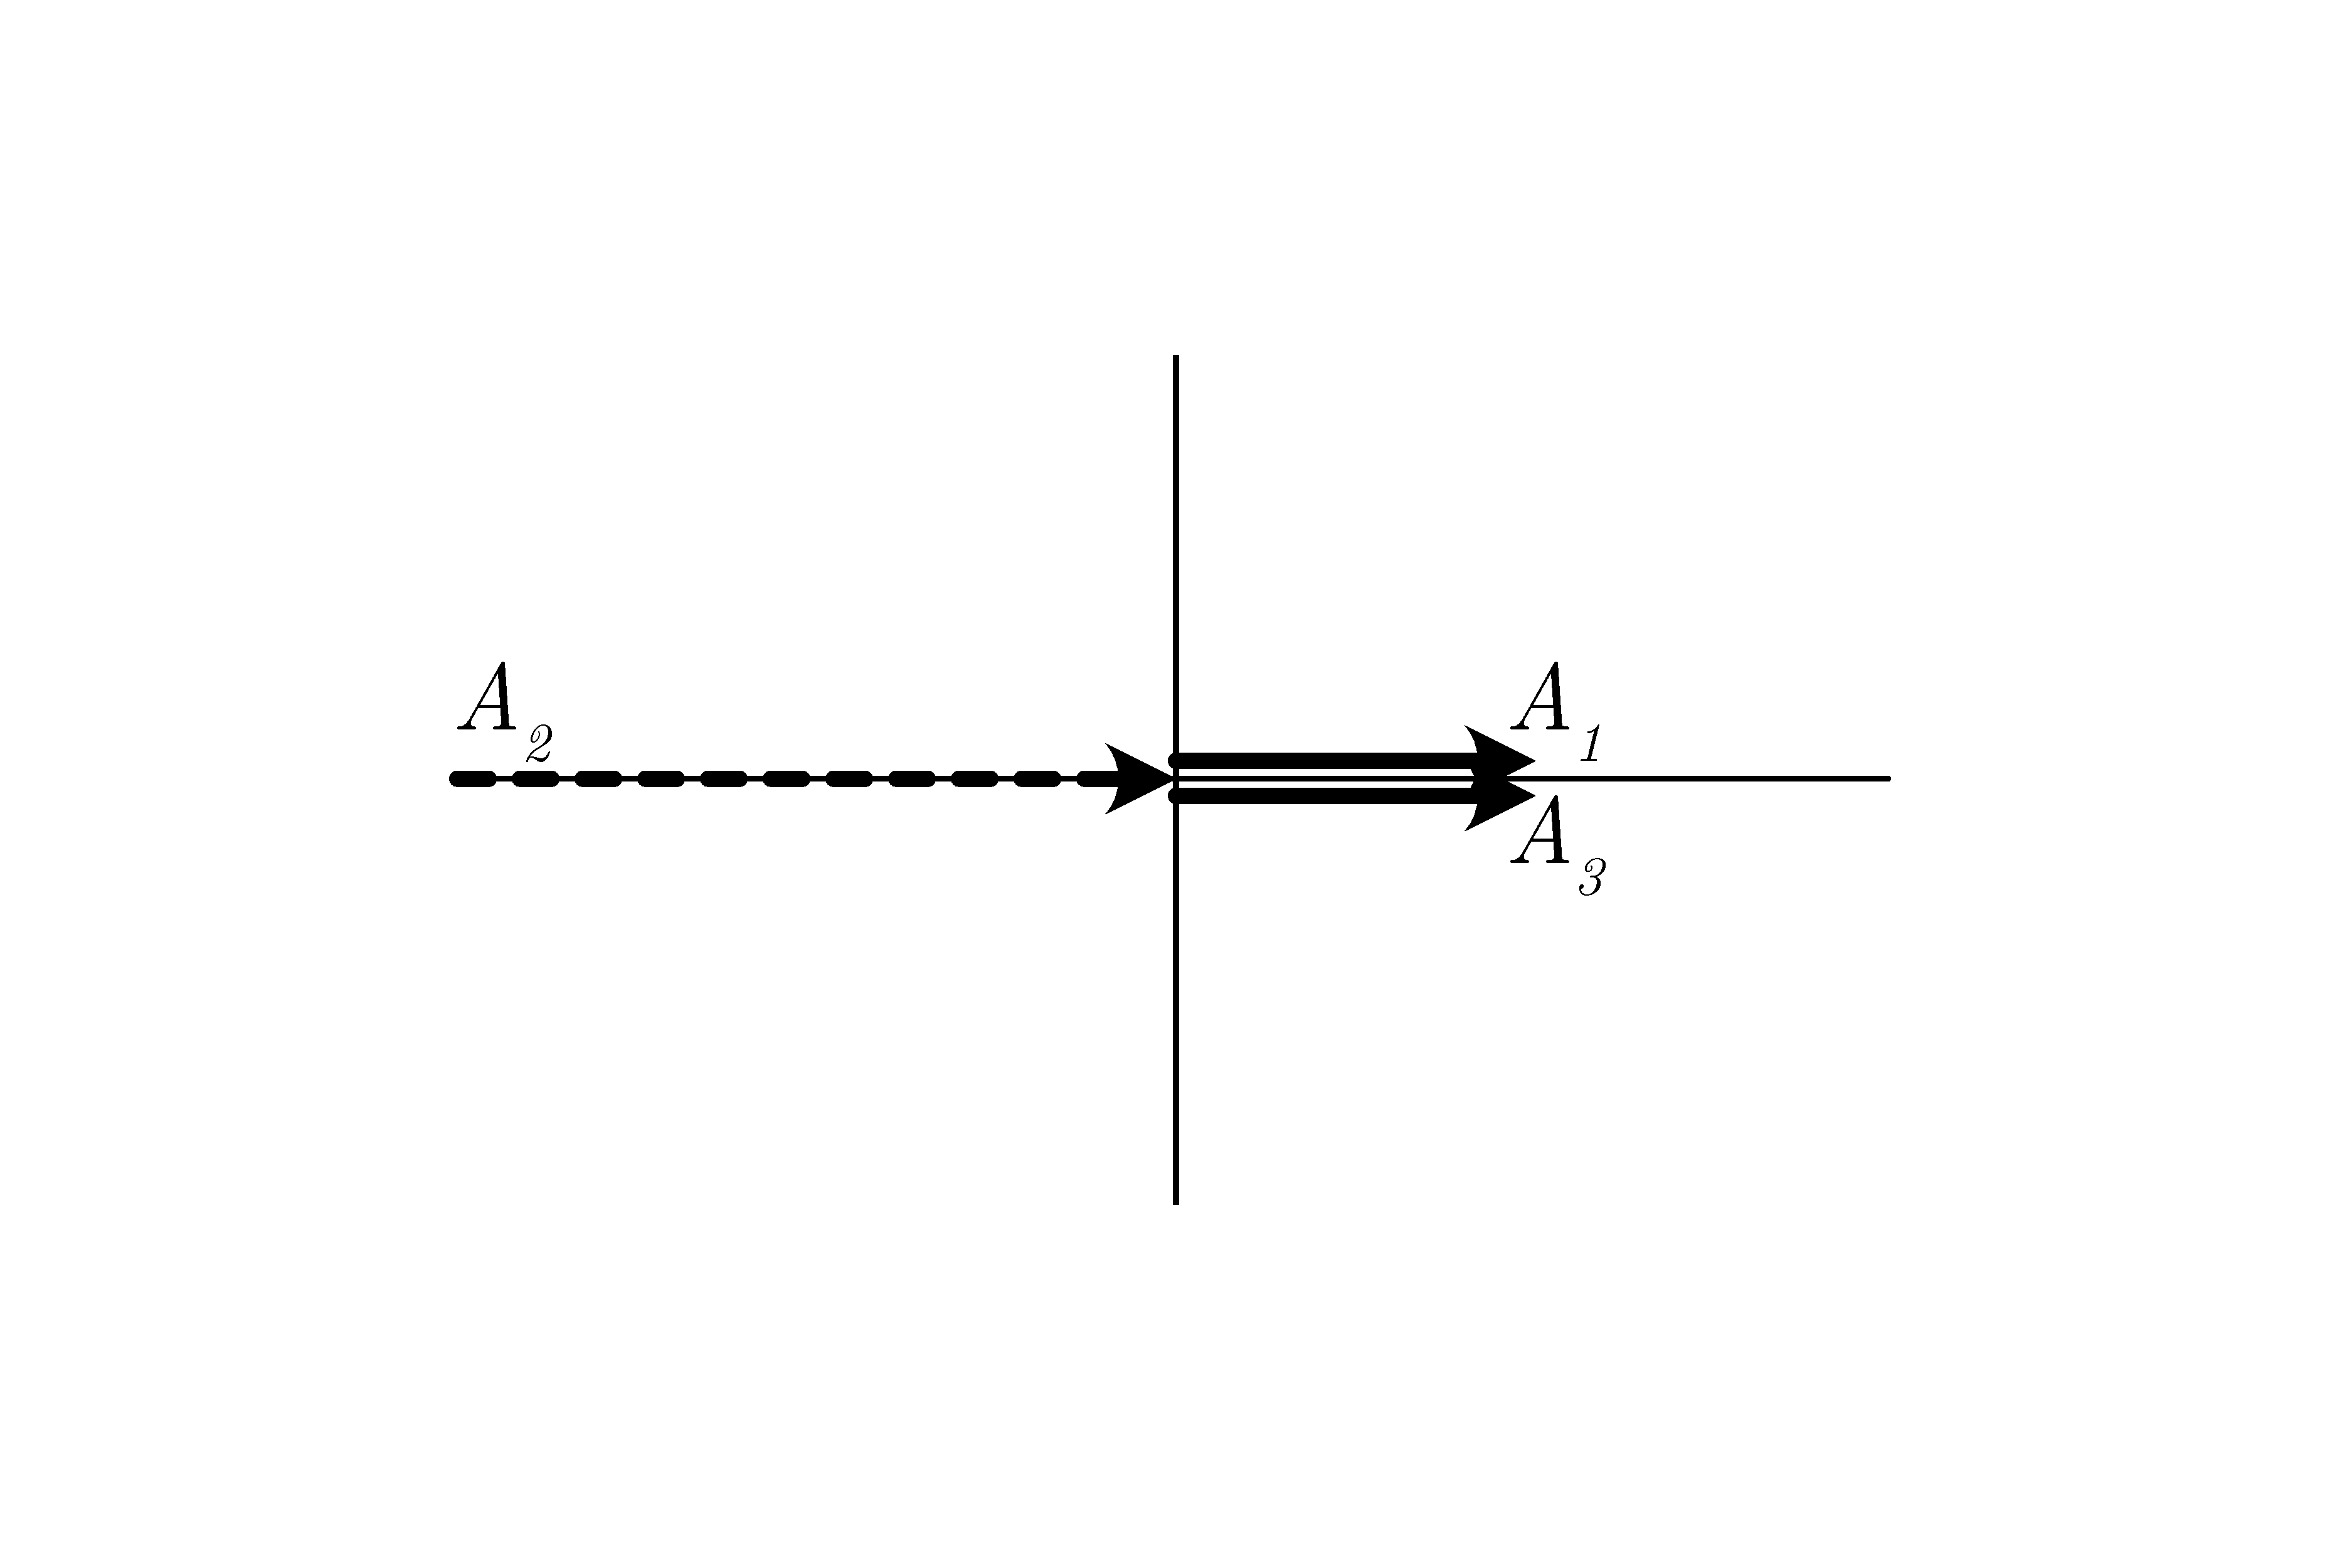
\includegraphics[width=\textwidth]{Figures/Ch3/input_shaping/bang_bang_vector}
    \caption{Vector Diagram}
    \label{fig:bang_bang_vector}
  \end{subfigure}
  \hfill
  \begin{subfigure}{0.3\textwidth}
    \centering
    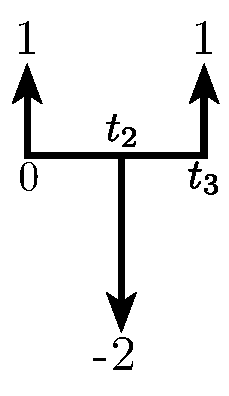
\includegraphics[width=\textwidth]{Figures/Ch3/input_shaping/bang_bang_impulses}
     \caption{Impulse Sequence}
     \label{fig:bang_bang_impulse}
  \end{subfigure}
   \caption{Maximum Vibration Bang-bang Impulse Sequence}
   \label{fig:bang_bang}
\end{figure} 

A vector diagram for a series of two bang-bang commands designed to maximize vibration is shown in Figure~\ref{fig:2x_bang_bang_vector}. This second bang-bang command in the sequence is just a repeat of the first, but beginning at time $\tau$, rather than at zero. The resulting impulse sequence is shown in Figure~\ref{fig:2x_bang_bang_impulse}
% 
\begin{figure}[tb!]
  \centering
  \begin{subfigure}{0.49\textwidth}
    \centering
    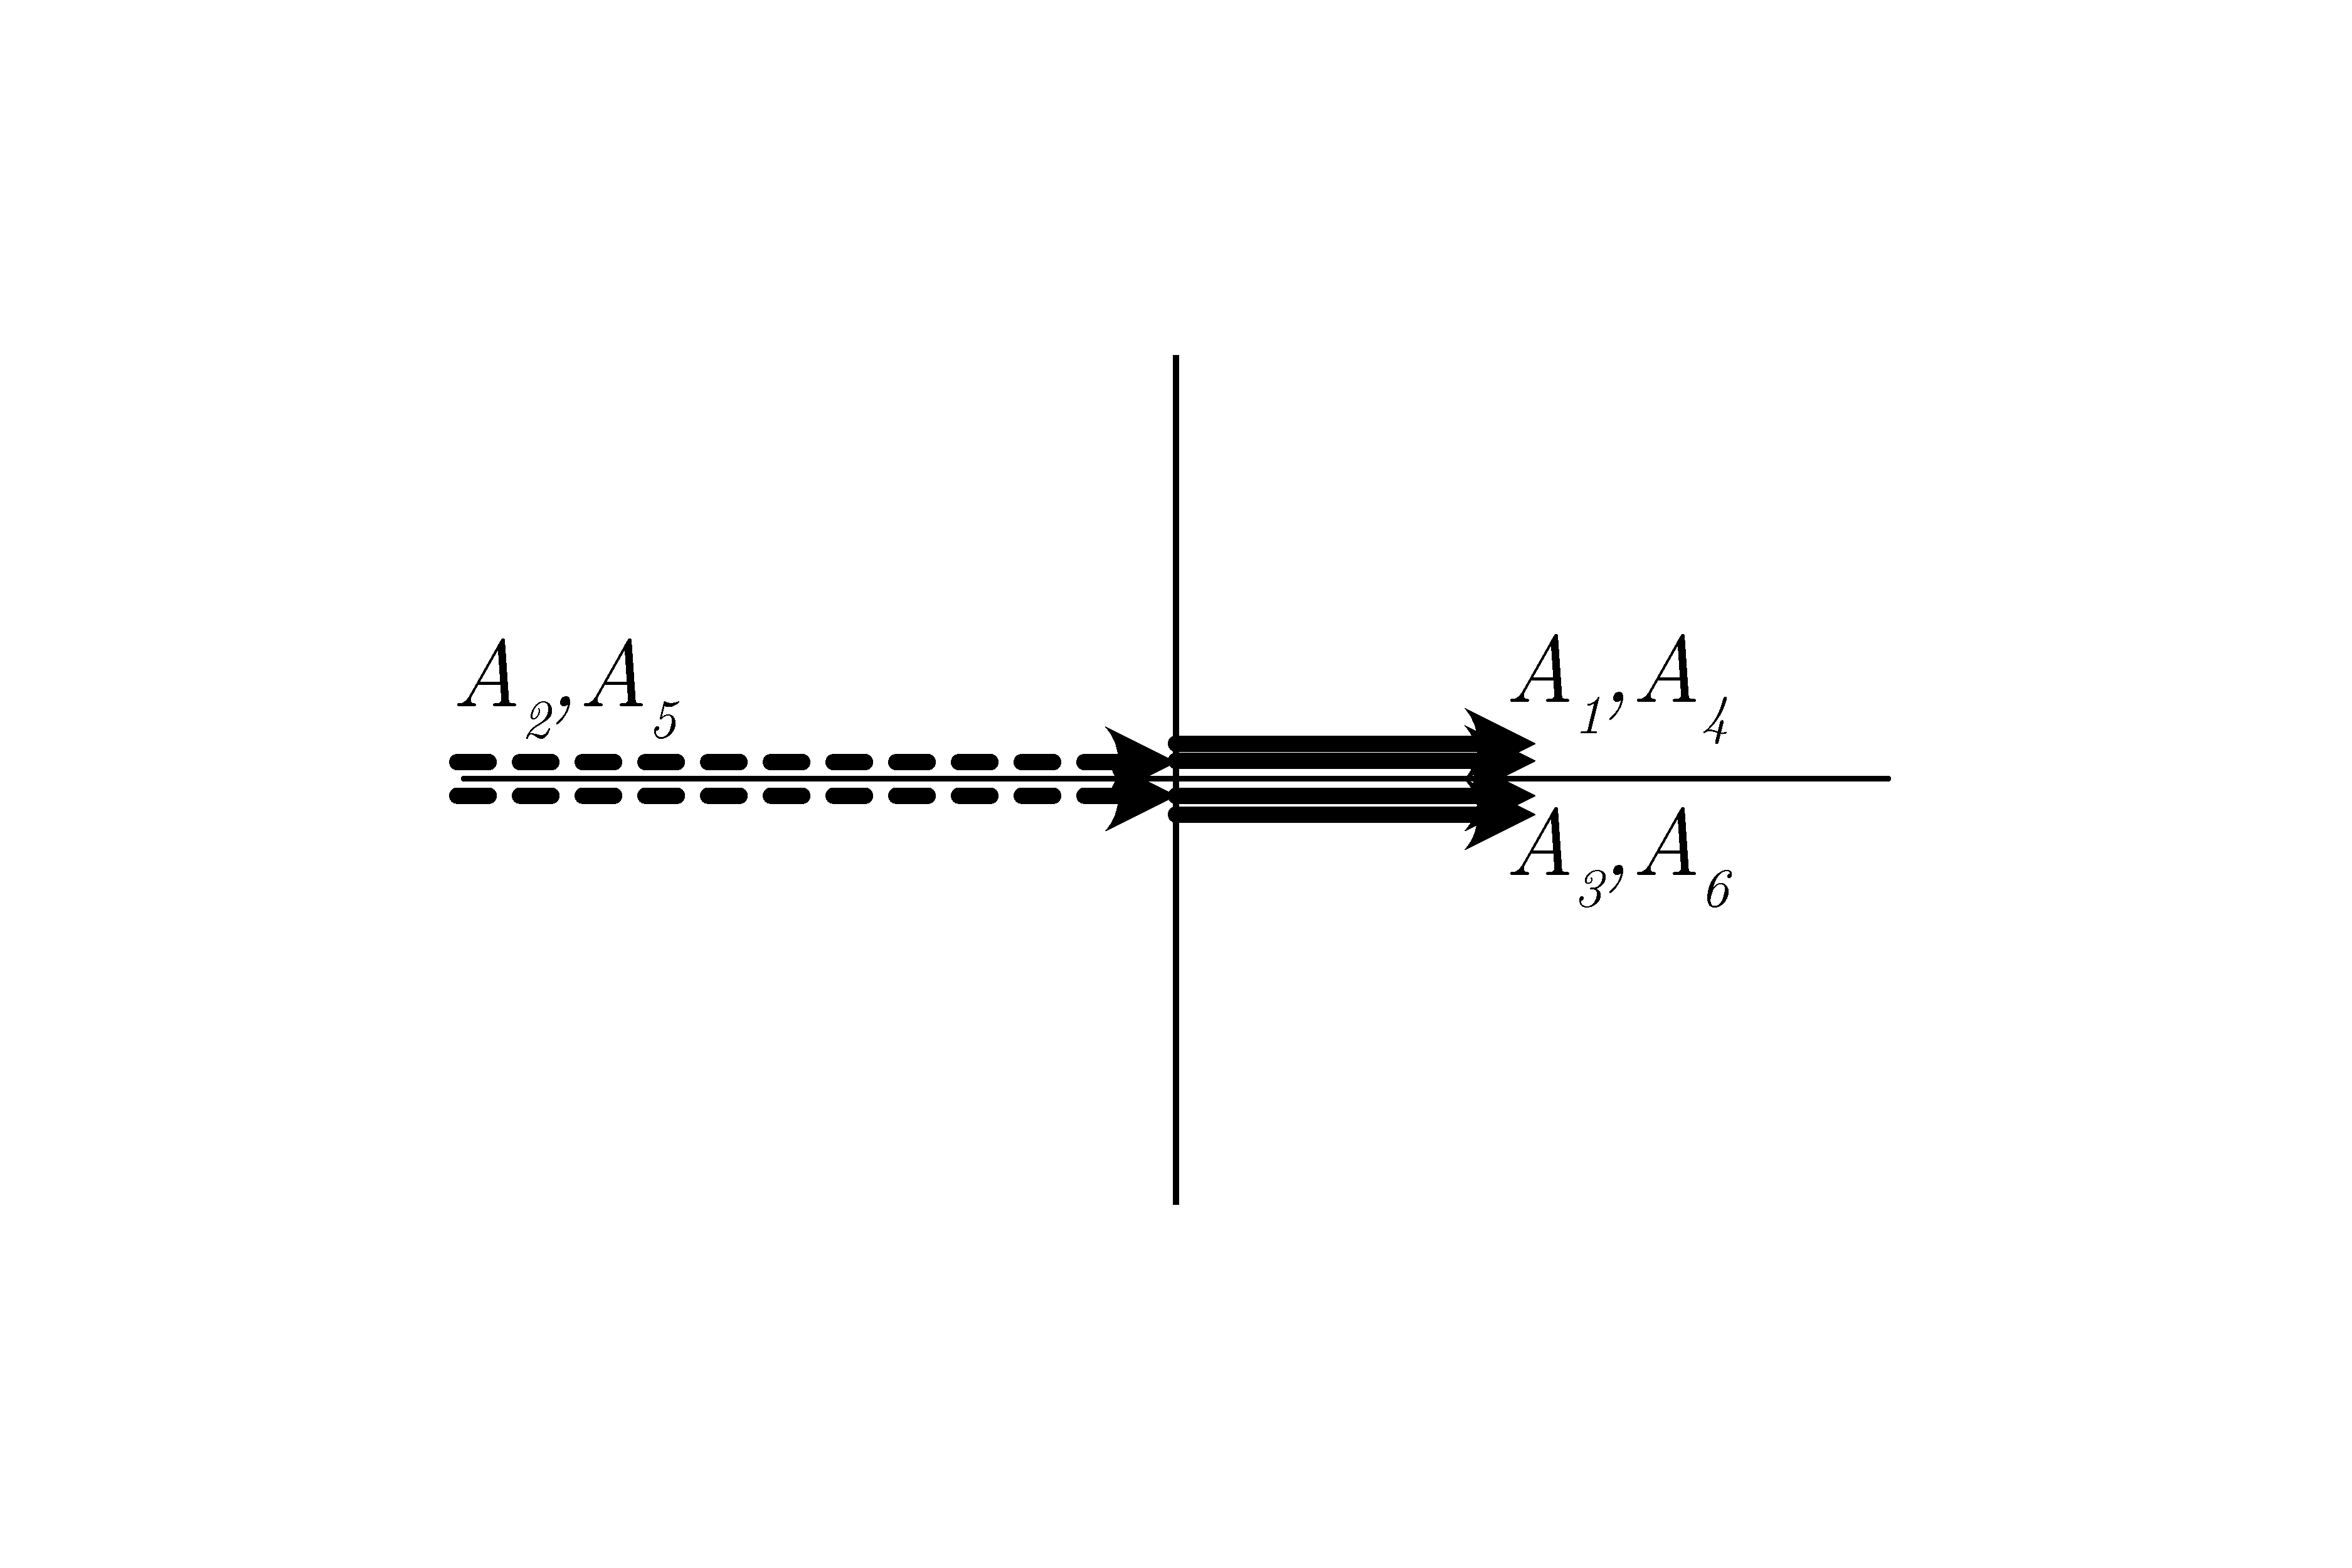
\includegraphics[width=\textwidth]{Figures/Ch3/input_shaping/2x_bang_bang_vector}
    \caption{Vector Diagram}
    \label{fig:2x_bang_bang_vector}
  \end{subfigure} 
  \hfill
  \begin{subfigure}{0.4\textwidth}
    \centering
    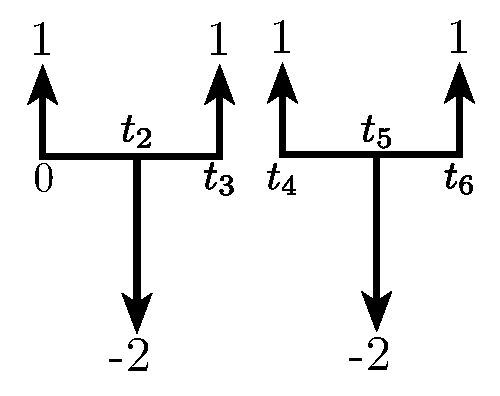
\includegraphics[width=\textwidth]{Figures/Ch3/input_shaping/2x_bang_bang_impulses}
     \caption{Impulse Sequence}
     \label{fig:2x_bang_bang_impulse}
  \end{subfigure}
   \caption{Maximum Vibration Dual Bang-bang Impulse Sequence}
   \label{fig:2x_bang_bang}
\end{figure} 
%
and can be written as:
\begin{equation}
\begin{bmatrix}A_i \\t_i\end{bmatrix} = \begin{bmatrix}1 & -2 & 1 & 1 & -2 & 1 \\[3pt] 0 & \frac{\tau}{2} & \tau & \tau & \frac{3\tau}{2} & 2\tau \end{bmatrix}
\label{eqn:2x_bang_bang_eq}
\end{equation}
%
where $A_i$ and $t_i$ represent the $i^{th}$ impulse amplitude and time, respectively. Given that the third and fourth impulses occur at the same time, the impulse sequence can further be simplified to:
%
\begin{equation}
\begin{bmatrix}A_i \\t_i\end{bmatrix} = \begin{bmatrix}1 & -2 & 2 & -2 & 1 \\[3pt] 0 & \frac{\tau}{2} & \tau & \frac{3\tau}{2} & 2\tau \end{bmatrix}.
\label{eqn:2x_bang_bang_eq_simple}
\end{equation}
%

The convolution of this impulse sequence with a step command in actuator acceleration, matching the process from Figure~\ref{fig:jumpConvolve}, is shown in Figure~\ref{fig:2x_bang_bang_conv}.
%
\begin{figure}[tb!]
\begin{center}
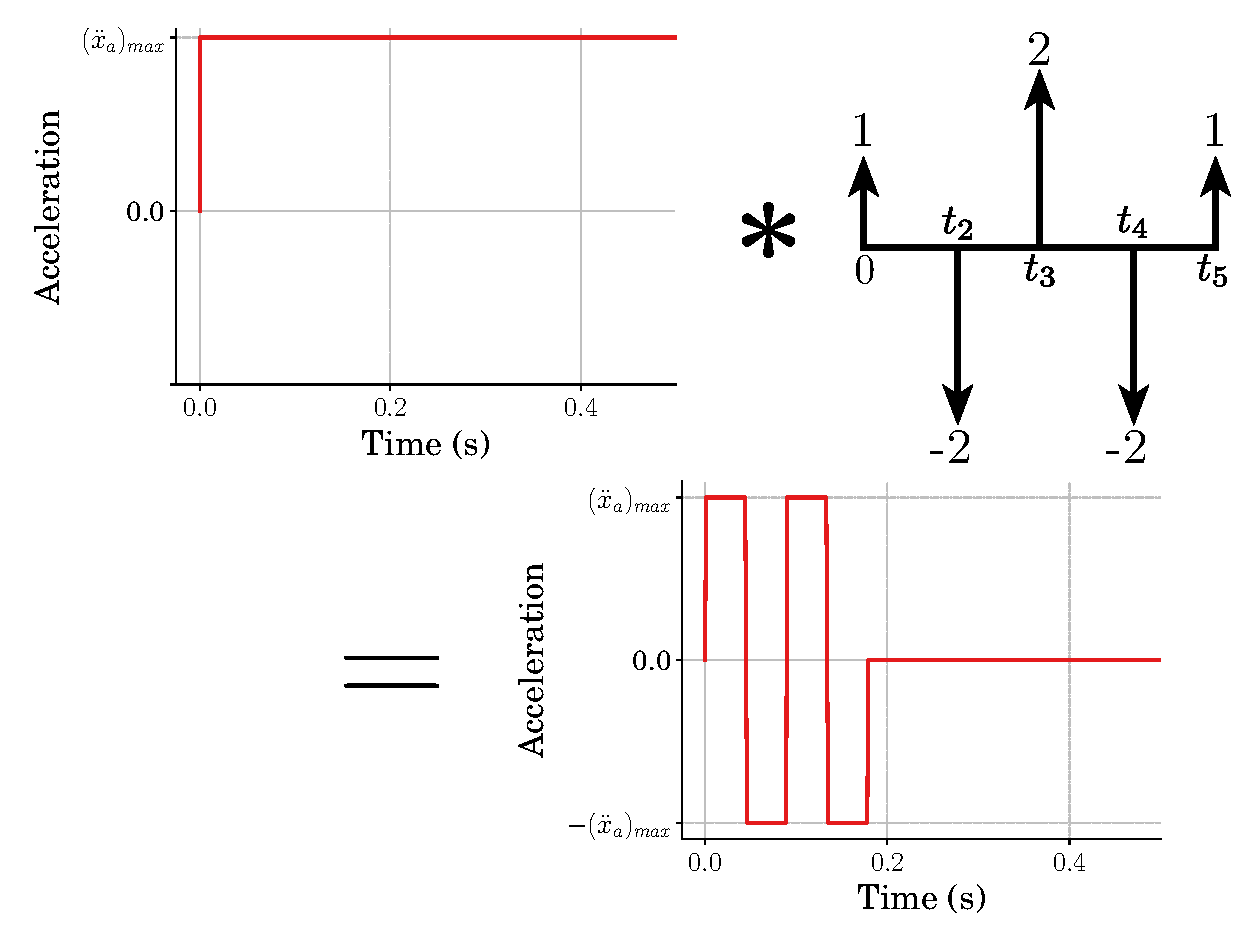
\includegraphics[width=0.85\textwidth]{Figures/Ch3/input_shaping/optimal_jump_convolve.pdf}  
\caption{Convolution of Maximum Vibration Bang-bang Impulse Sequence}
\label{fig:2x_bang_bang_conv}
\end{center}
\vspace{-0.2in}
\end{figure}
%
The resulting jumping response is shown in Figure~\ref{fig:optimum_jump} in comparison to the jumping response of the best high jumping agent from Chapter~\ref{chapter2}.
%
\begin{figure}[tb!]
  \centering
      \begin{subfigure}{0.49\columnwidth}
      \centering
      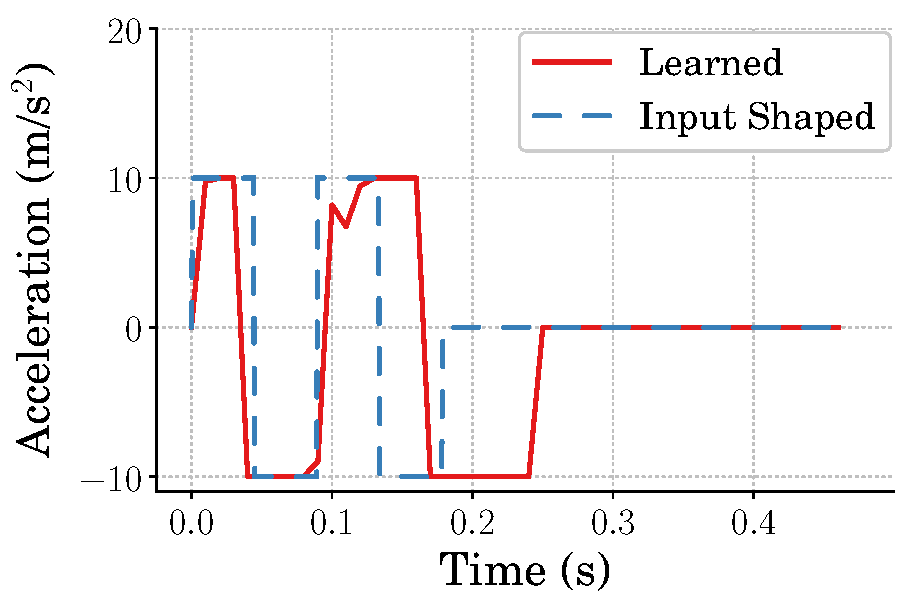
\includegraphics[width=\columnwidth]{Figures/Ch3/input_shaping/learned_comparison_to_optimal_command.pdf}  
      \caption{Jumping Commands}
      \label{fig:optimum_jump_command}
      \end{subfigure}
      \hfill
      \begin{subfigure}{0.49\columnwidth}
      \centering
      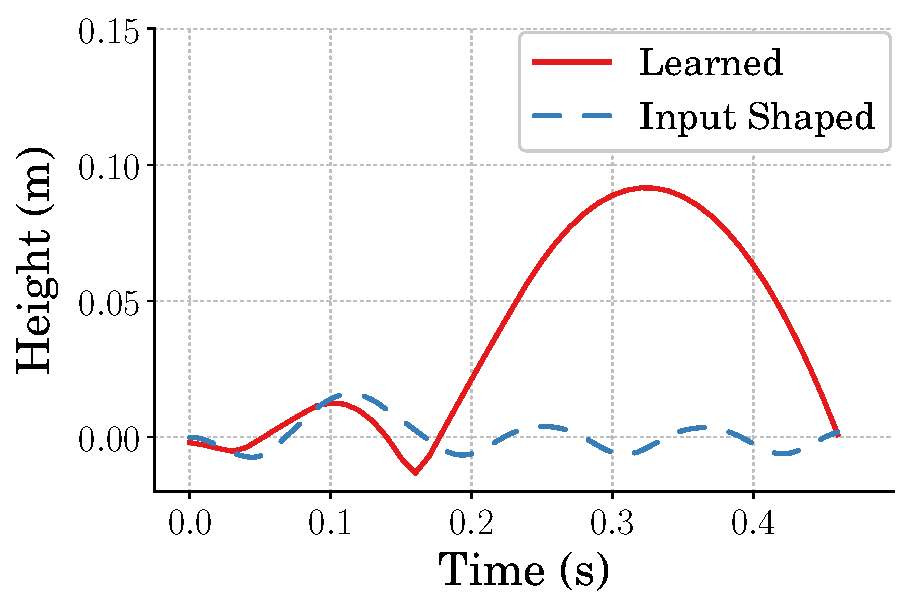
\includegraphics[width=\columnwidth]{Figures/Ch3/input_shaping/learned_comparison_to_optimal_response.pdf}  
      \caption{Jumping Responses}
      \label{fig:optimum_jump_response}
      \end{subfigure}
  \caption{Input and Jumping Response for Maximum Vibration Bang-bang Impulse Sequence} % Full figure caption
  \label{fig:optimum_jump}	% Full figure label
  \end{figure}
  %
This case represents the upper bound of the jump height possible for a linearized version of the monopode system, given the actuator limits imposed. While the form of the command in Figure~\ref{fig:2x_bang_bang_conv} is similar to that learned by the RL algorithm, shown in Figure~\ref{fig:opt_stutter_input}, the timing of the transitions between negative and positive acceleration are slightly different, particularly toward the end of the command. The input command, not having knowledge of the system through learning, fails to stutter jump the system. This happens as a result of the command timing not aligning with the position of the system. Looking at the timing in Figures~\ref{fig:optimum_jump_command} and~\ref{fig:optimum_jump_response}, it can be seen that the second positive acceleration ends too quickly without fully compressing the spring. With the spring not being fully compressed the system is still accelerating in the negative direction, so when the final negative acceleration is sent, the system simply decelerates and oscillates until the time limit is reached.

If the command learned by the agent in Figure~\ref{fig:opt_stutter_input} is analyzed directly, an impulse sequence representing its bang-bang profiles can be found to be:
%
\begin{equation}
\begin{bmatrix}A_i \\t_i\end{bmatrix} \approx \begin{bmatrix}1 & -2 & 2 & -2 & 1 \\[3pt] 0 & \frac{\tau}{2} & \tau & 2\tau & 3\tau \end{bmatrix}
\label{eqn:rl_match_impulses}
\end{equation}
%
A vector diagram of this sequence of impulses is shown in Figure~\ref{fig:rl_match_vector}. From the vector diagram, the resultant vector does not reach the amplitude of the theoretical upper-bound case, but does result in vibration that is 400\% of that which a single, unity magnitude impulse would create.
%
\begin{figure}[tb!]
\begin{center}
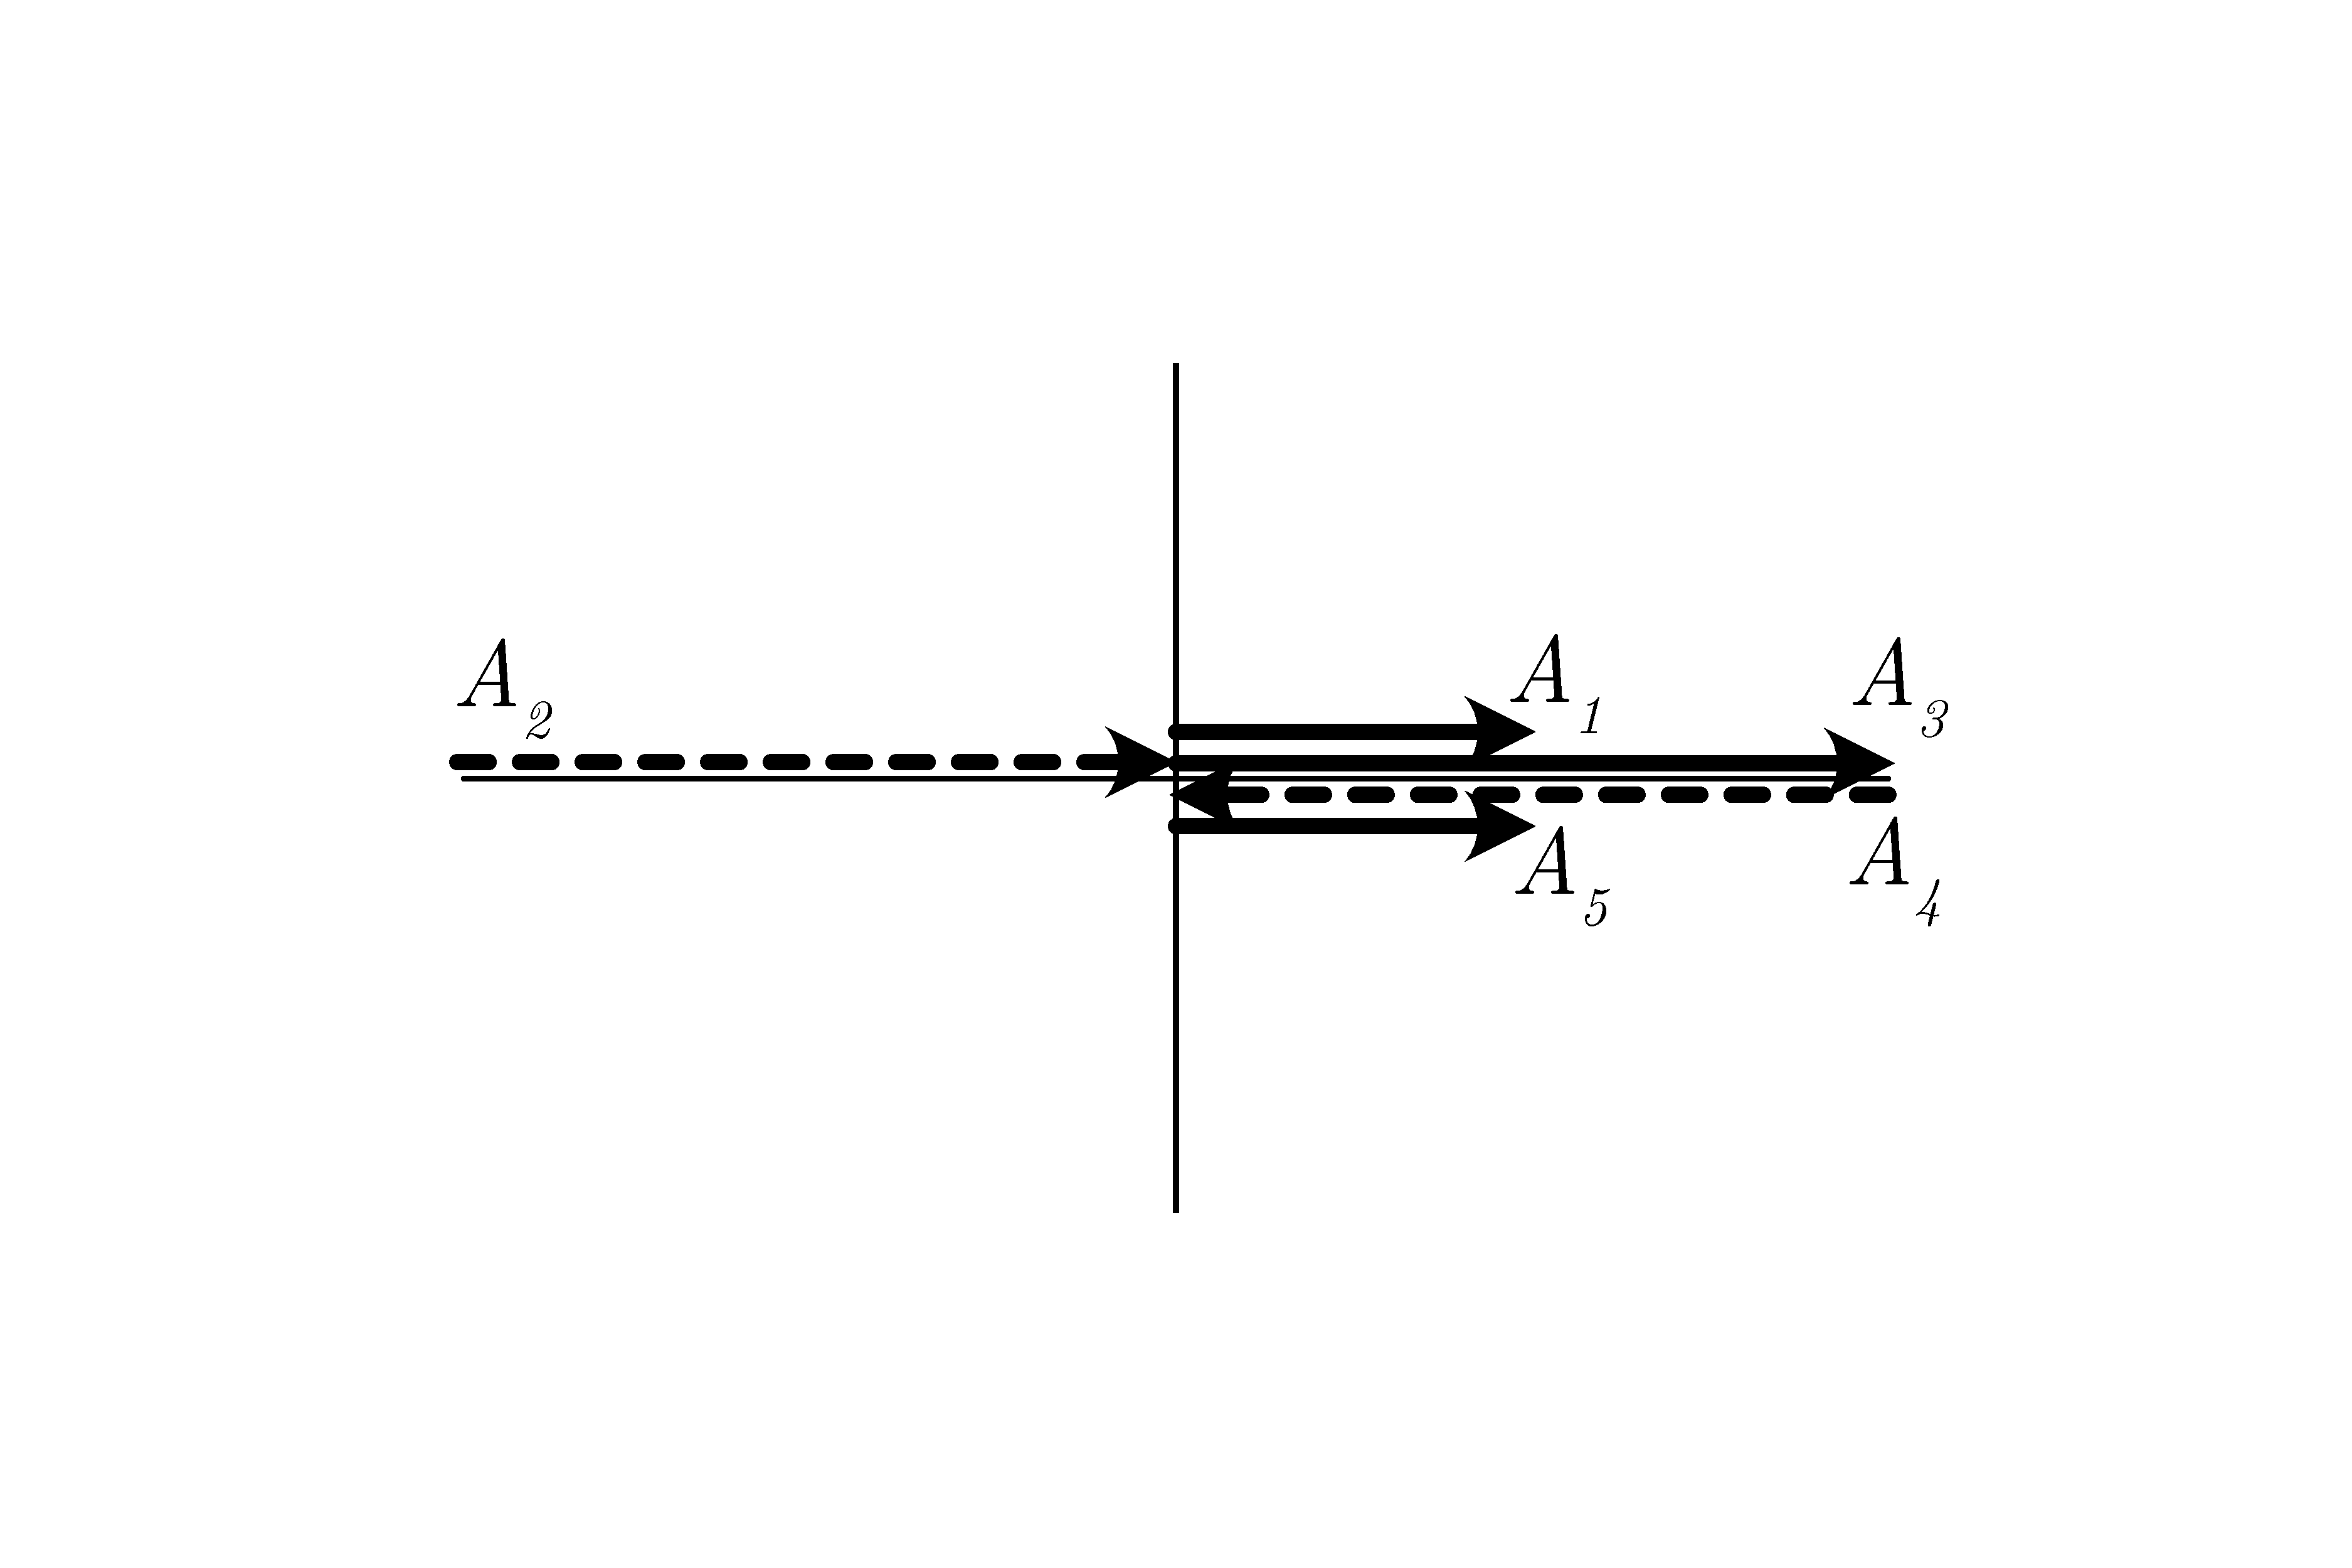
\includegraphics[width = 4in]{Figures/Ch3/input_shaping/rl_bang_bang_vector.pdf}
\caption{Vector Diagram for Learned Jumping Command}
\label{fig:rl_match_vector}
\end{center}
\vspace{-0.2in}
\end{figure}
%

The learned command and the one resulting from the convolution of this impulse sequence are shown in Figure~\ref{fig:learned_shaped_command_comparison}. The timing and amplitude of the command generated using the impulse sequence are a good match for the learned policy. This is further confirmed by comparing the jumping responses for the two commands, which are shown in Figure~\ref{fig:learned_shaped_response_comparison}.
%
\begin{figure}[tb!]
\centering
    \begin{subfigure}{0.49\columnwidth}
    \centering
    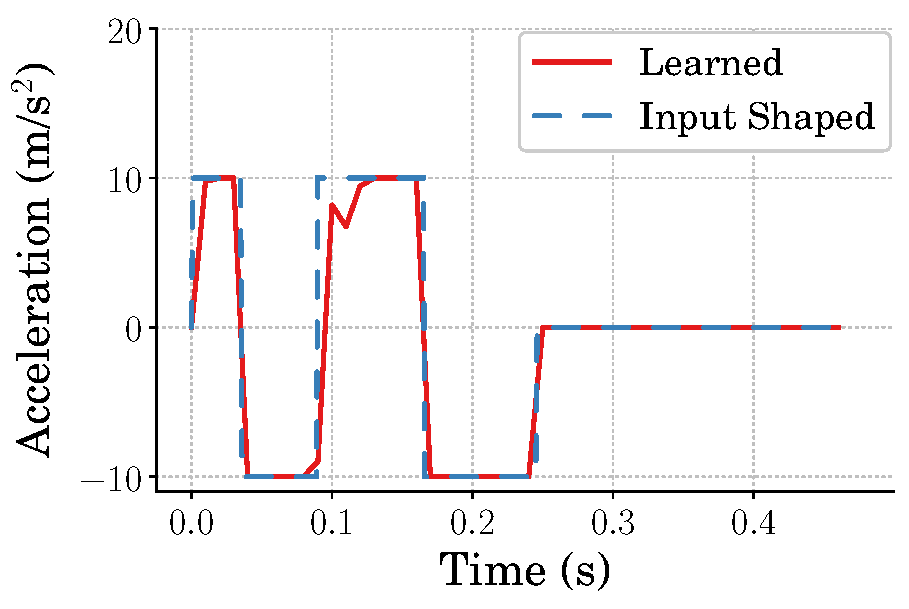
\includegraphics[width=\columnwidth]{Figures/Ch3/input_shaping/learned_shaped_command_comparison.pdf}  
    \caption{Jumping Commands}
    \label{fig:learned_shaped_command_comparison}
    \end{subfigure}
    \hfill
    \begin{subfigure}{0.49\columnwidth}
    \centering
    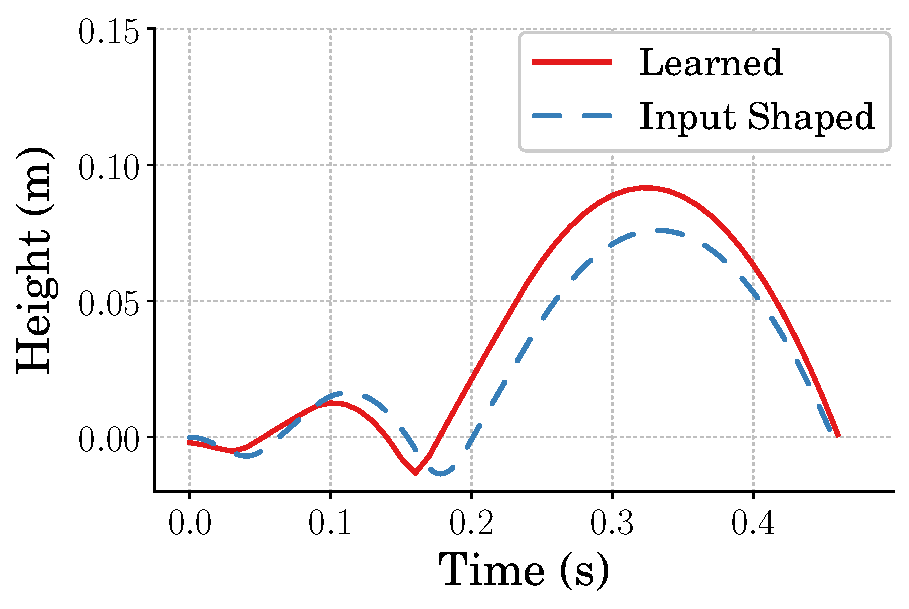
\includegraphics[width=\columnwidth]{Figures/Ch3/input_shaping/learned_shaped_response_comparison.pdf}  
    \caption{Jumping Responses}
    \label{fig:learned_shaped_response_comparison}
    \end{subfigure}
\caption{Comparison of Learned Controller and Input Shaping Approximation} % Full figure caption
\label{fig:rl_shaping_comparison}	% Full figure label
\end{figure}
%

In Figure~\ref{fig:learned_shaped_response_comparison}, the learned controller achieves a slightly greater jump height than the input-shaped approximation of it, but the general trends between the two match. The disparity in height is likely do to the input-shaped command being defined for a linear approximation of the monopode jumping system, whereas the RL-policy was trained on the nonlinear system. Both commands were evaluated on the nonlinear system. Regardless of the disparities, the results confirm that the methods presented in this chapter are a feasible option for analyzing control strategies learned using RL techniques.

%%%%%%%%%%%%%%%%%%%%%%%%%%%%%%%%%%%%%%%%%%%%%%%%%%%%%%%%%%%%%%%%%%%%%%%%
%%%%%%%%%%%%%%%%%%%%%%%%%%%%%%%%%%%%%%%%%%%%%%%%%%%%%%%%%%%%%%%%%%%%%%%%
\section{Conclusion}
%
An approach to design jumping commands using input shaping was reviewed. Then, the best learned stutter jumping command from Chapter~\ref{chapter2} was analyzed using methods approximating the command with an input-shaped step command. This analysis showed that the RL-learned command does not directly match the theoretical maximum for a linearized model of the monopode system. However, both the commands and responses for the shaped approximation and the RL agent matched closely, suggesting that input shaping is a feasible option for the analysis of learned policies.